\section{Related Work}

\subsection{Literature Search}

The search strategy was meticulously designed to ensure a comprehensive and thorough exploration of the literature concerning surgical tool tracking and related topics. The selected databases — PubMed and Ovid - are among the most comprehensive resources for biomedical literature, ensuring that the search covers a broad spectrum of relevant research. The literature search began in April, and to keep the review current, alerts were set up on PubMed to capture any newly published research. This ongoing search process, combined with backward and forward citation tracking and additional searches through other sources like Google Scholar, ensured that the review was as comprehensive and up-to-date as possible.

The Figure \ref{fig:prisma} illustrates the flow of the search and inclusion process, following the recommendations of the Preferred Reporting Items for Systematic Reviews and Meta-Analyses (PRISMA) statement \cite{moher_preferred_2010}. The strategy was divided into three main categories: tool-related searches, skill-related searches, and segmentation-related searches. This was not focused on conducting a systematic review but rather on establishing context, considering state-of-the-art (SOTA) methods and models, and identifying areas for further research in AI-enhanced laparoscopic training. This approach allows for a more flexible and comprehensive understanding of the current research landscape, facilitating the identification of gaps and opportunities for future research, including the focus for this study.

\begin{figure}[htbp]
    \centering
    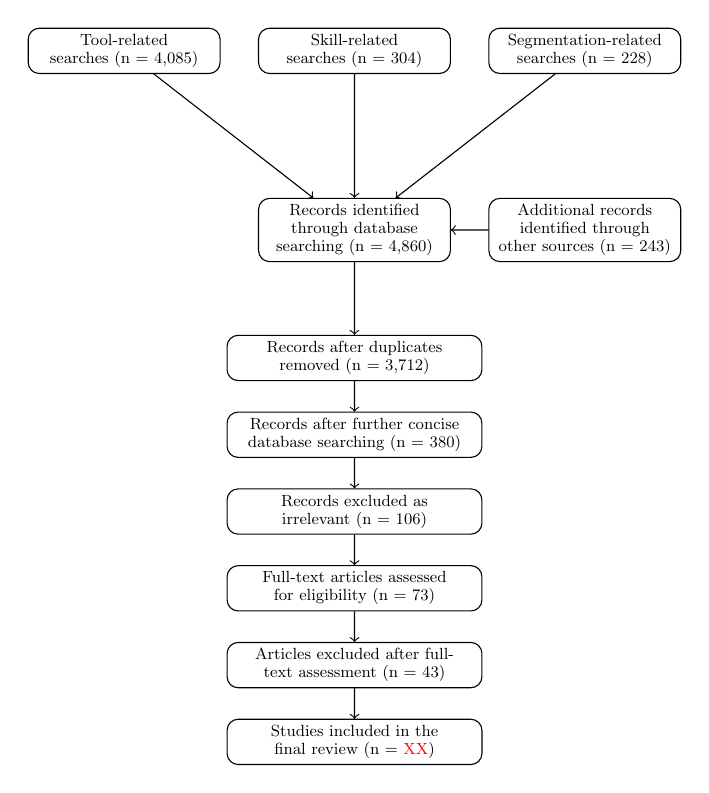
\begin{tikzpicture}[node distance=1.5cm, scale=0.65, every node/.style={transform shape, font=\fontsize{9}{10}\selectfont}]

    % Top level boxes
    \node (tool) [rectangle, draw, text width=10em, text centered, rounded corners] {Tool-related searches (n = 4,085)};
    \node (skill) [rectangle, draw, text width=10em, text centered, rounded corners, right of=tool, xshift=3cm] {Skill-related searches (n = 304)};
    \node (segmentation) [rectangle, draw, text width=10em, text centered, rounded corners, right of=skill, xshift=3cm] {Segmentation-related searches (n = 228)};

    % Box connecting to database searching
    \node (id) [rectangle, draw, text width=10em, text centered, rounded corners, below of=skill, yshift=-2cm] {Records identified through database searching (n = 4,860)};
    \draw[->] (tool) -- (id);
    \draw[->] (skill) -- (id);
    \draw[->] (segmentation) -- (id);

    % Additional records
    \node (os) [rectangle, draw, text width=10em, text centered, rounded corners, right of=id, xshift=3cm] {Additional records identified through other sources (n = 243)};
    \draw[->] (os) -- (id);

    % Duplicates removed
    \node (dup) [rectangle, draw, text width=13.5em, text centered, rounded corners, below of=id, yshift=-1cm] {Records after duplicates removed (n = 3,712)};
    \draw[->] (id) -- (dup);

    % Screening
    \node (sc) [rectangle, draw, text width=13.5em, text centered, rounded corners, below of=dup] {Records after further concise database searching (n = 380)};
    \draw[->] (dup) -- (sc);

    % Irrelevant exclusion
    \node (ex) [rectangle, draw, text width=13.5em, text centered, rounded corners, below of=sc] {Records excluded as irrelevant (n = 106)};
    \draw[->] (sc) -- (ex);

    % Full text assessed
    \node (ft) [rectangle, draw, text width=13.5em, text centered, rounded corners, below of=ex] {Full-text articles assessed for eligibility (n = 73)};
    \draw[->] (ex) -- (ft);

    % Articles excluded after full text assessment
    \node (fa) [rectangle, draw, text width=13.5em, text centered, rounded corners, below of=ft] {Articles excluded after full-text assessment (n = 43)};
    \draw[->] (ft) -- (fa);

    % Final studies included
    \node (inc) [rectangle, draw, text width=13.5em, text centered, rounded corners, below of=fa] {Studies included in the final review (n = \textcolor{red}{XX})};
    \draw[->] (fa) -- (inc);

    \end{tikzpicture}
    \caption{PRISMA Flow Diagram}
    \Description{The flow diagram of the paper selection and pruning process according to the recommendations of the PRISMA method.}
    \label{fig:prisma}
\end{figure}

\subsection{Identification and Evaluation of Relevant Datasets}

We identified 64 surgical datasets, of which we categorised 5 for tracking (where there is video access or subsequent frames available with appropriate annotations), 4 for pose estimation (with ground truth sensor data), 6 for detection (only bounding box annotations available), 10 for skill (classification of the operators' surgical skills), 11 for workflow analysis (the current sub-procedure or workflow carried out by the surgeon), 20 for segmentation (with full tool masks) and 7 for other use. Since some datasets have multiple use cases, we organised them so that if we could use them for tracking then we considered it to a dataset for tracking. In total, 37 datasets were identified as being useful with 9 excluded as they were based on robotic surgery (not relevant to us), with the remaning 18 datasets being excluded as they were not relevant. Only 7 datasets were ready for immediate use, with a further 5 available after requesting access.

Some datasets had more value as the quality of images and annotations were greater and very few had code available for direct use. We list these datasets as follows: MICCAI 2015 Endoscopic Vision Challenge (EndoVis 2015), MICCAI 2016 Endoscopic Vision Challenge (m2cai16), MICCAI 2024 Endoscopic Vision Challenge (SurgVU) \footnote{Based on the previous 2022 and 2023 challenge versions.}, PEg TRAnsfer Workflow Recognition by different modalities (PETRAW) \footnote{Sub-challenge as a part of MICCAI 2021} and the Augmented Reality Tool Network (ART-Net) dataset. Of these, the most relevant datasets were PETRAW as it is the ideal quality of the dataset that we would expect ours to be and ART-Net as it contained segmentation masks for tooltips which is something most datasets lacked.

% avoiding segmentation

% ART-NET: If there is enough time, we could try the method on another dataset. For ART-Net, we could convert the segmentation map into a bounding box, for the entire tool and just for the tool tip. I could consider other public datasets and what has been benchmarked already and how, so that I could employ the same method for comparison.

\subsubsection{Potential to Collect New Datasets}

% training datasets are fewer, easier to collect and to be used in LMIC

\subsection{State-of-the-Art Object Detection Methods}

% emphases what has been done

% Anchor-based is interesting because videos often have a wide range of aspect ratios, etc. (insert examples). We decided that it would be best to continue with the current dataset, and to make it scientific and sufficient for the MSc, I would look at investigating anchor-based methods (e.g. YOLO) and anchor-less methods (fully connected one-stage CNN). A method for each would be sufficient. The idea is that the aspect ratio of the tool will change as it moves around and is rotated, with different orientations and scales in various ways, so anchors in anchor-based methods would need to be optimised. I would look at what methods could cope with those situations and what their limitations are.

% Many Deep Learning based methods such as Fast-RCNN have achieved SOTA performance in tool detection and localization (Du et al, 2018a) but are computationally expensive, introducing inference time penalties. https://arxiv.org/abs/2209.01435

We can use RetinaNet with anchor-box optimisation \cite{zlocha2019improving}.

\subsection{Tracking Methods}

% Secondary focus is tracking, the main focus is on detection. Tracking can be done if IDs are tracked and we consider tools moving out of frame (their appearance, disappearance and reappearance). Segmentation is not needed as tracking is our aim, not pixel-wise classification.

% many different algorithms, and list some (DeepSORT, ByteTrack, BotSORT) however we will create our own algorithm for us on datasets similar to PETRAW and our dataset.

\subsubsection{Computer Vision Methods}

There are many alternative methods which can be used for specific tasks, which can be incredibly useful with increasing accuracies of detection and tracking. Optical flow methods estimate the motion of objects between consecutive frames of video. By tracking keypoints or pixels, these methods can determine movement patterns which correspond to the movement of the tool. A key technique used in the Lucas-Kanade method which utilises a differental method for optical flow estimation, efficient for small motion which is what we experience in laparoscopic data. It also uses the Horn-Schunkck method which assumes smoothness in the motion field. This works well in real-time applications and can be used to track movement across frames with moderate accuracy. We can improve the robustness and accuracy by using sensor data to initialise and help guide the optical flow tracking process. The Kalman Filter method is an extremely popular and widely used method in tracking which provides estimates of unkown variables by optimally combining a series of measurements observed over time, which is excellent for real-time applications and noisy data. A particle filter can track the tool positions based on probabilistic models, based on sensor readings and a motion model. This makes it robust to non-linearities and multi-modal distirbutions in the sensor data. Background subtraction is a simple method which involves separating foreground objects from the background in video frames to isolate and track moving objects. We can use Gaussian Mixture Models to model the background using multiple normal distributions to adapt to changes in lighting, scene dynamics and camera movement. The simplest methd is to use frame differencing to highlight moving objects. This is extremely effective in controlled environments with static backgrounds making it highly suitable in our application. Feature matching can be used to track movement by detecting and matching key features such as corners and edges. With enhancemnets such as speeded-up robust features (SURF), a faster alternative to scale-invariant feature transform (SIFT) which describes local features, we can track keypoints in real-time applications, robust to scale and rotation changes common in laparoscopic videos. We could use template matching where we use pre-defined templates of the tools to locate and track frame-by-frame. Its weakness is in aspect-ratio changes which can be countered by also implemeneting one of the aforementioned SIFT or SURF techniques. Simple edge detection and contour tracking can also be used in non in-vivo datasets where there is a simpler non-moving background compared to in-vivo data.

\subsubsection{Artificial Intelligence Methods}

Artificial intelligence methods can be used to track tools in laparoscopic videos. We can use a deep learning method such as a convolutional neural network (CNN) to detect tools in images. Then we can use a recurrent neural network (RNN) to use previous information to help reinforce predictions in the current frame. We coudl also use a long short-term memory (LSTM) network to remember information over long periods of time, or a gated recurrent unit (GRU) network which is a simplified version of an LSTM network which is more efficient and can be used in real-time applications. We could use a transformer network which is a deep learning model that uses attention mechanisms to learn dependencies between input and output data. 
All of these methods essentially allow us to track tools in real-time applications, with the ability to learn from previous frames and predict future frames.

\subsection{Potential Gaps and Insights}

% what has not been done whicih could be done
% pose research questions

\subsection{Limitations}

\subsection{Future Use Cases}

% Need to have a concise plan going forward. I have focused on image tracking and segmentation across many datasets. Going forward, I should consider what could be done, working with state-of-the-art (SOTAs) and focusing on something different to give different results. Using the papers from the literature review I have carried out, I should pick a paper, run the SOTA method and consider why it performs best or why it fails at certain things. These things are where I should look for improvements. Consider the mistakes made and how I could solve them. If there are good and bad samples, then focus on those which fail and innovate on what could be done about them. For example, there could be different sizes or occlusions or look at the domain-safe problem (solving the generalisation problem on real and fake data). If the methods do not work on real data, what is the gap which needs to be solved? Goal is to get inference down.